\documentclass[10pt]{beamer}
\usepackage[utf8]{inputenc}
\usepackage[T1]{fontenc}
\usepackage{tikz}
\usepackage{pgf-pie}
\usepackage{pgfplots}
\usepackage{booktabs}
\usepackage{tabularx}
\usepackage{xcolor}
\usepackage{adjustbox}

\pgfplotsset{compat=1.18}
\usetikzlibrary{positioning}

% Cores P&G
\definecolor{pgblue}{RGB}{0,84,159}
\definecolor{pglightblue}{RGB}{64,131,214}
\definecolor{pgdarkblue}{RGB}{0,48,95}

% Configurações do Beamer
\setbeamercolor{structure}{fg=pgblue}
\setbeamercolor{normal text}{fg=pgdarkblue}
\setbeamertemplate{navigation symbols}{}
\setbeamertemplate{footline}[frame number]
\setbeamersize{text margin left=1cm,text margin right=1cm}

\begin{document}

%% CAPA PERFEITA (ajustada para não sobrepor)
\begin{frame}[plain]
\begin{tikzpicture}[remember picture,overlay]
  % Faixa azul
  \fill[pgblue] (current page.south west) rectangle ([xshift=3.5cm]current page.north west);
  
  % Conteúdo
  \node[white,anchor=west,xshift=4cm,yshift=2cm] at (current page.west) 
    {\Huge\textbf{FEMIBION}};
    
  \node[white,anchor=west,xshift=4cm,yshift=1.2cm] at (current page.west) 
    {\Large Brazil Market Entry};
    
  \node[anchor=west,xshift=4cm,yshift=0.3cm] at (current page.west) 
    {\large\textcolor{pgdarkblue}{Brief Financial Plan for Femibion}};
    
  \node[anchor=west,xshift=4cm,yshift=-0.5cm] at (current page.west) 
    {\small\textcolor{pgdarkblue}{2022}};
\end{tikzpicture}
\end{frame}

%% SLIDE 2 - OBJETIVOS FINANCEIROS
\begin{frame}{Financial Targets}
\vspace{-0.5cm}
\begin{block}{Core KPI}
\begin{tabularx}{\textwidth}{lXX}
\toprule
\textbf{Metric} & \textbf{Target (12mo)} & \textbf{Growth} \\
\midrule
Brand Share & 0.6\% & +100\% \\
Revenue & R\$26.9M & +99.3\% \\
Market Value & R\$12.8B & +2.4\% \\
\bottomrule
\end{tabularx}
\end{block}

\begin{tikzpicture}[remember picture,overlay]
\node[anchor=south east,xshift=-5mm,yshift=5mm] at (current page.south east) 
{\tiny\textcolor{pgblue}{Source: Internal P\&G Data 2022}};
\end{tikzpicture}
\end{frame}

%% SLIDE 3 - ALOCAÇÃO DE INVESTIMENTO
\begin{frame}{Investment Allocation}
\centering
\scalebox{0.9}{
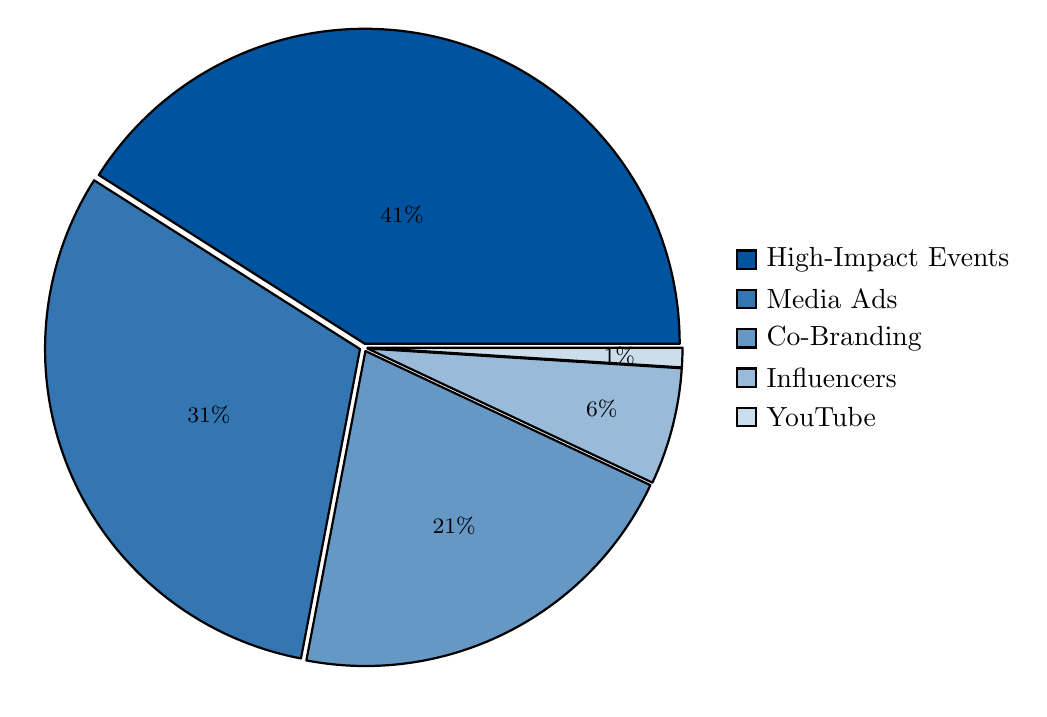
\begin{tikzpicture}
\pie[
    radius=4,
    explode=0.05,
    text=legend,
    color={pgblue,pgblue!80,pgblue!60,pgblue!40,pgblue!20},
    before number=\footnotesize,
    after number=\%
]{
    41/High-Impact Events,
    31/Media Ads,
    21/Co-Branding,
    6/Influencers,
    1/YouTube
}
\end{tikzpicture}
}

\begin{itemize}
\item \textcolor{pgblue}{\textbf{72\%}} Budget to high-ROI channels
\item \textcolor{pgblue}{\textbf{R\$3.5M}} Tactical marketing
\end{itemize}
\end{frame}

%% SLIDE 4 - PROJEÇÕES
\begin{frame}{Revenue Forecast}
\centering
\vspace{-0.5cm}
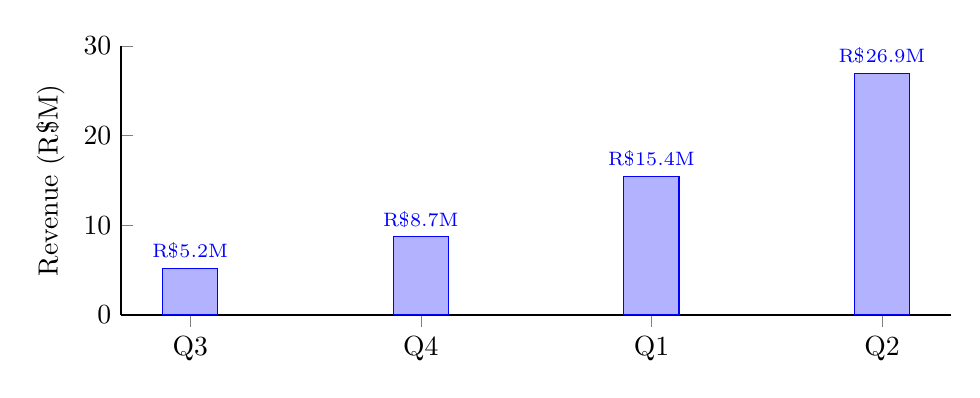
\begin{tikzpicture}
\begin{axis}[
    ybar,
    width=\textwidth,
    height=5cm,
    bar width=0.7cm,
    symbolic x coords={Q3,Q4,Q1,Q2},
    xtick=data,
    nodes near coords={\scriptsize R\$\pgfmathprintnumber{\pgfplotspointmeta}M},
    ymin=0,
    ymax=30,
    ylabel={Revenue (R\$M)},
    axis lines*=left,
    every axis plot/.append style={fill=pgblue}
]
\addplot coordinates {(Q3,5.2) (Q4,8.7) (Q1,15.4) (Q2,26.9)};
\end{axis}
\end{tikzpicture}

\begin{exampleblock}{}
\centering Projected \textcolor{pgblue}{\textbf{518\% growth}} from Q3'22 to Q2'23
\end{exampleblock}
\end{frame}

%% SLIDE 5 - ANÁLISE DE RISCO
\begin{frame}{Risk Matrix}
\framesubtitle{Market Entry Challenges}

\centering
\begin{tikzpicture}[scale=0.85, transform shape]
\draw[fill=pgblue!10, thick] (0,0) rectangle (10,4);

\foreach \y/\percent/\text in {3/75/Economic, 2/42/Regulatory, 1/21/Competition, 0/10/Supply} {
    \draw[fill=pgblue!(100-\percent), thick] (0,\y) rectangle (0.1*\percent,\y+1)
      node[midway, white, align=center] {\textbf{\text}\\\percent\%};
}

\node[anchor=west] at (10.2,3.5) {\scriptsize • Inflation • FX rates};
\node[anchor=west] at (10.2,2.5) {\scriptsize • ANVISA • Taxes};
\node[anchor=west] at (10.2,1.5) {\scriptsize • Natuvit • Private labels};
\node[anchor=west] at (10.2,0.5) {\scriptsize • Logistics • Costs};
\end{tikzpicture}
\end{frame}

%% SLIDE FINAL
\begin{frame}{Conclusion}
\centering
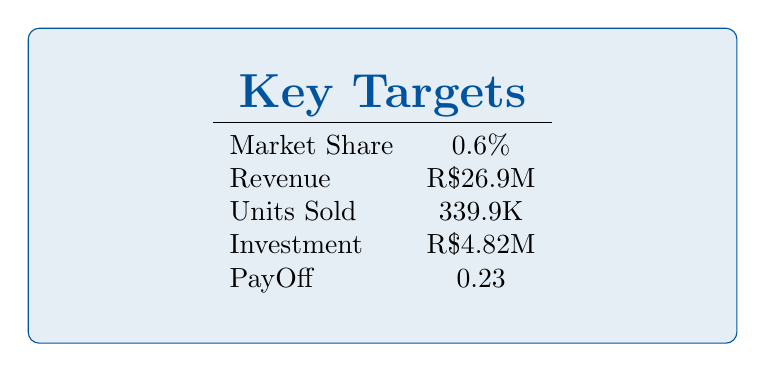
\begin{tikzpicture}
\node[draw=pgblue, fill=pgblue!10, rounded corners, minimum width=9cm, minimum height=4cm] {
\begin{tabular}{lc}
\multicolumn{2}{c}{\LARGE\textcolor{pgblue}{\textbf{Key Targets}}} \\
\midrule
Market Share & 0.6\% \\
Revenue & R\$26.9M \\
Units Sold & 339.9K \\
Investment & R\$4.82M \\
PayOff & 0.23 \\
\end{tabular}
};
\end{tikzpicture}

\begin{tikzpicture}[remember picture,overlay]
\node[anchor=south east,xshift=-5mm,yshift=5mm] at (current page.south east) 
\end{tikzpicture}
\end{frame}

\end{document}